%!TEX root = ../main.tex
\section{System Analysis} % (fold)
\label{sec:system_analysis}
A thorough system analysis is needed in order to design an embedded system that meets the needs expressed by the use cases. 
This section will present the analysis of the complete embedded system, through the following topics:

\begin{itemize}
\item Parameters of interest. The use cases do not describe what parameters should be monitored meaning that it should be investigated which are relevant to monitor.
\item Hardware for monitoring parameters. It should be analysed what hardware is necessary in order to measure the parameters found to be relevant. 
\item Amount and frequency of data????. Something clever about this. Martins sections should be used for it.
\item Data collection. It should be analysed how data is collected on the go-kart.
\item Micro-controller. It should be analysed what micro-controller should be used on the go-kart.
\item Wireless network. It should be analysed how data is transferred from the go-kart 	to the stationary computer.
\item Local storage. There needs to local storage on the go-kart and it needs to be analysed what kind this should be and how it should be implemented.
\item UI. It should be be analysed how the transferred data should be presented to the user in an UI.
\end{itemize}

\subsection{Parameters of Interest}
\label{sec:parameters}
In developing new hardware or evaluating current hardware, it is necessary to be able to monitor a range of parameters.
This section will investigate what parameters need to be logged in order to provide a useful and complete logging of the behavior of the go-kart.
The parameters in question fall into three categories; Physical parameters, electrical parameters and mechanical parameters.
These will be dealt with in turn in the following sections
\paragraph*{Physical Parameters}
This category comprises all information about the motion of the go-kart.
\begin{itemize}
	\item \textbf{Position, Absolute:} Providing a means to record the absolute position of the go-kart is a useful feature in certain fields.
	Especially any form of localisation and path finding will be able to put this information to use.
	The absolute position of the go-kart can be recorded using a GPS module or possibly by using a known starting coordinate and information about the relative movement of the go-kart.
	\item \textbf{Position, Relative:} The relative position of the kart can be, as just mentioned, used to infer the absolute position of the go-kart.
	Additionally it can provide a means to analyze a drivers performance on track the or detect drift while cornoring.
	The relative position includes both translational, as well as rotational information.
	This information can be gathered using an inertial measurement unit (IMU).
	An IMU is a compound device, comprising of an accelerometer and a gyroscope and, in some cases, a magnetometer.
	\item \textbf{Velocity:} The velocity of the go-kart is key in optimising lap-times, clearly, it is desirable to monitor this parameter.
	It can be extracted by reading the motor encoders.
	However, the driving wheels are prone to slippage when cornoring, this would give an inaccurate reading of the actual velocity of the go-kart.
	Instead, a simple encoder can be mounted on either one, or both of the front wheels as these are freerunning and independent.
	Once the rotational speed of the axle is known, the velocity of the go-kart can be infered using the tyre diameter.
	\item \textbf{Acceleration:} It may be of interest to monitor the forces exerted on the go-kart, or, its acceleration, as it drives on the track.
	This information is already provided by the accelerometer in the IMU mentioned above and as such provides no additional complication.
\end{itemize}
Three sensors are mentioned in this section.
A GPS, an IMU and an encoder.
In order to limit the scope of the project only the GPS and the IMU will be implemented.
\paragraph*{Electrical Parameters}
This category comprises all information about the electrical aspects of the go-kart.
\begin{itemize}
	\item \textbf{Motor Currents:} Providing a means of monitoring the currents flowing through the motor allows the user to calculate the torque exerted by the motor as well as the current power draw of the motor.
	Knowing the currents could also prove an invaluable debugging tool when developing a new inverter for the go-kart.
	\item \textbf{Throttle Position:} The throttle on the go-kart is connected to a potentiometer.
	Measuring the voltage output of this potentiometer provides a simple way of monitoring the position of the throttle.
	\item \textbf{Desired Currents:} Based on the current throttle position a set of desired currents are calculated.
	Monitoring these allows spotting any discrepancies between the desired and the actual currents.
	\item \textbf{Duty Cycles:}
	\todo[inline]{Mikkel: What do you mean?}
	\item \textbf{Battery Voltage:} As the go-kart is electrical, naturally, it has a battery.
	Monitoring the current battery status could give the user an indication of how much driving time is left, or how long until the batteries are recharged afterwards.
	\item \textbf{Motor Angle:} Knowing the angle of the motor at all times gives a means of more accurately calculate the currents at specific times.
	Additionally, it can be used in Clarke-Parke transformations, again, providing information in debugging an inverter in development.
\end{itemize}
These parameters are all available from the sevcon gen4 motor controller mounted on the go-kart.
This controller has a CANopen interface from which this data can be extracted.
Any users who wish to add their own inverter will simply need to obey the API stated by the sevcon gen4 CANopen interface in order to correctly log the data.
\paragraph*{Mechanical Information}
This category comprises all information about the mechanical aspects of the go-kart.
\begin{itemize}
	\item \textbf{Steering Wheel Angle:} Monitoring the angle of the steering wheel allows analysing the performance of the driver.
	In addition it opens up for the possibility of mechanical control of the go-kart.
	Similarly to monitoring the velocity, the steering wheel angle can be monitored by adding an encoder to the steering column.
	\item \textbf{Braking Pedal Position:} The braking system on the go-kart is similar to that of an ordinary car.
	The braking disc is mounted on the driving axle and the braking calibers connected to the brake pedal by a series of oil-filled hoses.
	Monitoring its actuation allows analysing the performance of the driver and as mentioned above, may potentially allow for mechanical control of the go-kart
\end{itemize}
As both of these parameters would require mechanical changes to the go-kart, they are beyond the scope of this project and as such will not be implemented.
\subsubsection*{Conclusion}
In this section a multitude of different parameters have been discussed.
Most of them can be logged using just three components; a Sevcon Gen4 motor controller, an IMU and a GPS.
These are the three components from which data logging will be implemented throughout this project.
This provides a solid platform to prove the concept and additional sensory equipment can be added at a later date, should it be required.


























\subsection{Hardware for Monitoring Parameters}
\label{sec:hardware_for_par}
In section \ref{sec:parameter} an overview of the different parameters that may be of interest for logging is given.
It was concluded that three components would suffice as a proof of concept; the Sevcon Gen4 motor controller, an IMU and a GPS.
This section will explore in more detail what requirements and communication schemes exists for each of the components.

\subsubsection*{Sevcon Gen4 Motor Controller}
\todo[inline]{Mikkel: Something here?}

\subsubsection*{Inertial Measurement Unit (IMU)}
IMU's, generally, exist in two versions.
A 6D and a 9D version.
Both include an accelerometer and a gyroscope.
In addition to these the 9D IMU includes a magnetometer, enabling measurement of absolute direction, as opposed to the relative measurement of direction granted by the magnetometer.
The requirement in terms of each of these parts is given as:
\begin{itemize}
	\item \textbf{Accelerometer [\si{\metre\per\second^2}]:} As the name implies, the accelerometer measures accelerations.
	That is, when the component changes speed or direction the force exerted on the accelerometer is measured.
	Professional drivers using professional grade go karts driving upwards of 250 \si{\kilo\metre\per\hour} can reach up to 2-3 g's of force exerted on them.
	The go kart available in this project has a theoretical maximum speed of 50 \si{\kilo\metre\per\hour}.
	Clearly, the forces exerted on this platform will be lower, however, a minimum requirement of $\pm$ 3g will be set for the accelerometer in the IMU.
	\item \textbf{Gyroscope [\si{\degree\per\second}]:} 
\end{itemize}
\todo[inline]{Mikkel: Which one do we chose?}

\subsubsection*{Global Positioning System (GPS)}
\todo[inline]{Mikkel: Something here?}


\subsubsection*{Conclusion}
\todo[inline]{Table with chosen sensors and their interfaces}









\subsection{Network}
We need to write something about that we chose to have a local on-vehicle network and a wireless network.

Monolithic?










\subsection{Data Logging}
\todo[inline]{Mikkel: Should maybe change name?}
A feature will be data logging. 
Any data could be put into the log, although some signals can be logged at significantly higher rates than others
If all data is recorded at the fastest rate, this could present a storage problem.
This challenge will be analyzed here.
\subsubsection{Sample Rate}

Datalogging should be useful for working with an inverter as was the case on the first semester.
Likely it would be interesting to log the phase-current to the motor at high enough rate to accurately depict their sinusoidal short term average.
The ripple current or voltage at the motor terminals should be measured in the lab, as this requires a high sample rate, and more control than offered on the test track.
This data logging would be useful for recording current in the motor as the go kart is driving.
Additionally it would be relevant to record the encoder output, and possibly the DC voltage at the input of the inverter and the duty for each phase.
Only the currents are bound to change rapidly, and as such they determine the minimum acceptable sample rate.
By looking at the maximum frequency of the motor and the most extreme rate of change permissible by the armature inductance, it is possible to set a sample rate for the log file.\\

According to the manufacturer of the motor, the maximum rotational velocity is 5000 RPM.
With four pole pairs, this comes to a maximum sinusoidal frequency of 333 Hz. 
It is not necessary to record at a rate significantly larger than the Nyquist limit in order to adequately record the sinusoidal.
Simulations show, that by using Clark-Park transformation, interpolation and then the inverse Clarke-Park transformation, there is nearly no difference between a low sample rate of $1\si{\kilo\hertz}$, and a higher sample rate of $3.3\si{\kilo\hertz}$, as shown below.

\begin{figure}
	\centering
	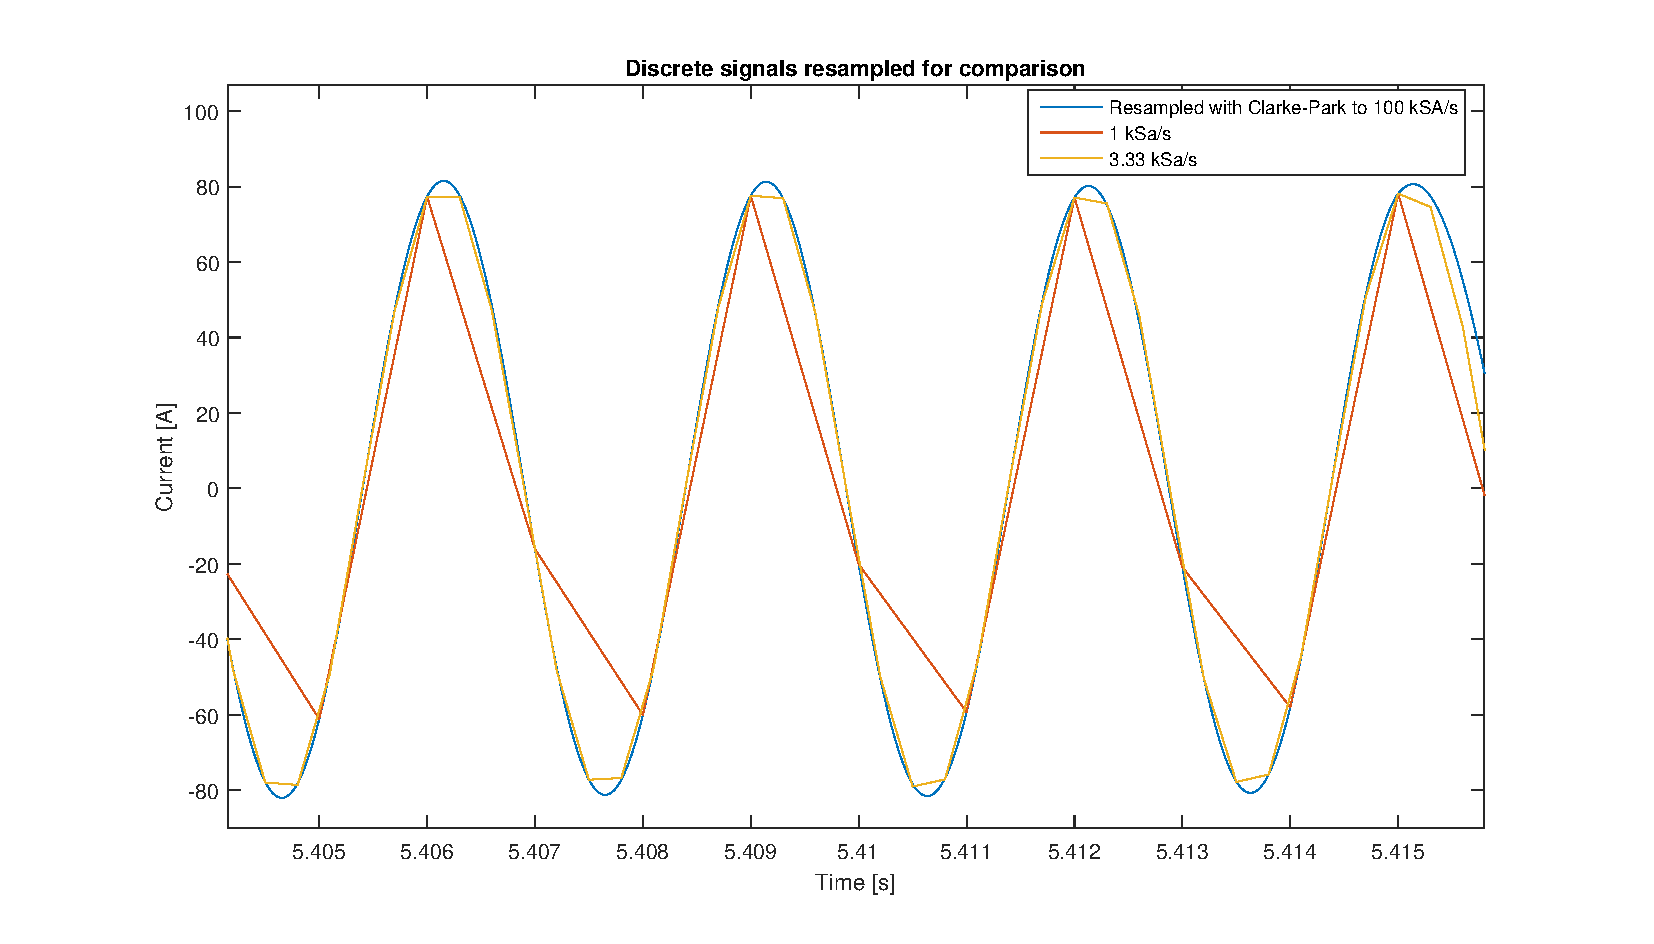
\includegraphics[width = 0.9\linewidth]{graphics/Clarke-park_resampled}	
	\caption{Comparison of data recorded at 1 kSa/s and 3.33 kSa/s, against 100 kSa/s resampled using Clarke-Park}
	\label{fig:Clarke-park_resampled}
\end{figure}

The resampled data from the 1 kSa/s and 3.3 kSa/s (orange and purple respectively on figure\ref{fig:Clarke-park_resampled}) are almost identical.
However, there is a small visible difference around the time 5.527 s, likely due to the limited precision of the encoder.
This also doesn't take into account any disturbance or noise, which could make it hard to reconstruct the signals with lower sample rates.\\

Additionally, the Matlab function, resample, produces nicely filtered vectors with smaller time steps, so it is possible to use a low sample rate for time invariant signals.\\
Another way to look at this is to calculate the maximum change in current from one sample to another.
This is determined by the inductance of the motor, which is $600 \si{\micro \henry}$ \todo[inline]{when one half bridge is high, and the two others are low, it's one armature inductance of 400 uH in series with two parallel armature inductances}, and the maximum voltage across it, which is $V_{BAT}=52.8 \si{\volt}$. 
At a sample rate of 3.33 kSa/s, this results in a theoretical maximum step of $264\si{\ampere}$.
A sample rate lower than this, would make it hard to properly record such sudden steps.

\subsubsection{Data Type}
When the sample rate is known, it is possible to get an estimate of how much storage space would be needed. 
It would be easiest, and most useful, to record using simple comma separated files, but these tend to take up more space than necessary.
The analog input to the Zybo are 12 bit, which means, that full precision of these would be possible with 4 digits, and often a decimal point and potentially a negative sign.
Including the horizontal separator, this comes to 6.5 bytes per point.\\

An example of recording could include time, two currents, a voltage and the encoder output, as displayed below
\begin{lstlisting}
Time	Ia	Ib	V	Encoder
1.0000	052.3	-278.1	52.56	16
1.0003	057.7	-280.4	52.54	17
\end{lstlisting}
That brings each line length to 32 bytes (8 bytes for time, 5.5 for the three analog, 3 bytes for encoder, 5 for separators).
At a sample rate of 3.33 kSa/s, this comes to 6.1MB per minute. 
With the current SD cards having 4 GB of free un-partitioned space, this gives up to 11 hours of recording time.\\

Alternately, it is possible to invent a file structure, that allows several arrays of with different data types.
By storing numbers in binary files instead of text, it is possible to reduce the space requirements to a third (2 bytes per analog, 4 bytes per timestamp (allowing up to 49 days of ms), and 1 byte for encoder).
This however will reduce the readability greatly, and include the workload, as one will need to write code both for encoding and decoding the file. \\

Since this is out of the scope of this project, and the sample rate isn't larger than it is, logging in standard ASCII will suffice.
Likely, different sample rates will be recorded to different log files












\subsection{Micro-controller}
As described in section \ref{sec:data_collection} there should be a CAN network of nodes on the go-kart.
Each node is a sensor or other data producing unit along with a micro-controller.
From the perspective of the network the only requirement for the micro-controller is that it has a CAN controller.
In principle the network could consist of 16 different micro-controllers.

\subsubsection*{Sensor Nodes}
As described in section \ref{sec:hardware_for_par}, it was chosen to use an IMU and a GPS with a USB interface. 
As specified in the use cases one of the nodes needs to transfer data wirelessly from the go-kart to the stationary computer. 
Both USB interface and wireless data transfer drivers are implemented in operating systems like Linux, Mac OS X and Windows.
Thus choosing a micro-controller supporting such an operating system will greatly simply the code that needs to be written for those sensor nodes.
Developing software for Linux is a part of a course that the group is attending therefore Linux will be used as the operating system.
\\
The Zybo board will be used for the sensor nodes as it has a built-in CAN controller, it has the ability to run Linux and the group has access to it.

\subsubsection*{Zybo Board}
The Zybo board has a Xilinx Zynq Z-7010 chip, which has a processing system (PS) part and a programmable logic (PL) part.
The PS consists among other of a dual-core ARM Cortex-A9 processor and I/O peripherals including CAN and USB.
The PL consists of a Xilinx 7-series Field programmable gate array. 
The PL and PS are connected through a bus called AXI.
The Zybo board itself is a developing platform consisting, among other, of several buttons, switches, LEDs and connections for USB, Ethernet, HDMI and several PMOD connectors.


\subsubsection*{Linux on the Zybo Board}
Several Linux distribution are configured to run on the Zybo board. 
The group has experience with a the Xillinux \footnote{http://xillybus.com/xillinux} distribution, therefore this will be used.
Xillinux is based upon the Xilinx distribution witch is based upon Ubuntu 12.04.
In the Xillinux architecture there is a bus between the PL and PS named Xillybus.
Xillybus is implemented as an IP core in PL and a corresponding Xillybus driver in the Xillinux kernel.
In PL the IP core is interfaced through standard FIFO buffers and the Xillybus is reached in userspace through \textit{"/dev/xillybus\_"}.
\todo[inline]{Mikkel: Check this path on Zybo.}

\subsubsection*{Conclusion}
Nodes on the network need not to be a specific micro-controller, they just need to able to use CAN.
The Zybo board running Xillinux will be used for IMU, GPS and wireless network node to ease development as Linux includes both USB and network drivers. 


\subsection{Data Collection}
\label{sec:data_collection}
\todo[inline]{Mikkel: Needs to be rewritten!}
\subsubsection{Topology}

There are various network topologies that can be used to setup the required node network for this project.
These include the ring, bus, mesh ,star and tree topology. Before we specify which one is suitable, a brief description of the purpose and functionality of our network as well as an overview of their advantages and disadvantages are needed. 

\paragraph{Purpose of the Network}~\\
\todo{Add the abbreviation ov = on-vehicle somewhere somehow}
The purpose of this network is to accommodate multiple nodes, such as sensors sub-networks and in general data-producers.
These need to be able to communicate with the main on-vehicle computer as well as among them.
The reasons for this is that the ov-computer is responsible for transmitting and receiving data from the stationary computer and other nodes may require data from other nodes to cooperate for a task.
Also, the ov-computer, apart from communicating, will also handle processing that the rest of the nodes are not able to. 
\\\\
The communication between the various nodes does not require a central hub.
Two nodes may need to communicate with one another without the control and the extra processing time of a centralized topology.
Furthermore, in the case that one fails, the network as a whole should still be operative.
Lastly, since it is a multi-node network and it may require more nodes in the future, a certain level of scalability is also required.

\paragraph{Different Topologies}~\\
\begin{itemize}
\item \textbf{Bus:} This is the simplest and cheapest topology.
All nodes communicate through a central bus and it is scalable with the addition of extra nodes on the two ends of the cable.
The central bus introduces the risk of complete network failure in case of the bus failure and the decrease in performance in case of many nodes or heavy traffic.
\item \textbf{Ring:} All the nodes in this type of network form a ring, where each node is connected to its two neighbors.
It has the advantages of the bus network as well and it shows better performance, even under heavy load.
A centralized control is not required for this type and in case of a node failure, the ring breaks and it can continue to function as a bus network.
It is scalable, but to a less extent than the bus.
\item \textbf{Mesh:} In this type, each node has direct connections to each other node present in the network.
That provides speed and reliability in case of node failures, but requires more hardware and processing power to manage the connections.
It is very robust but scalability is certainly not one of its features.
\item \textbf{Star:} The star topology is a centralized type of networking.
All nodes are connected to a central hub, handling all the communication between them.
It is fast, easy to implement and offers great reliability in case of node failures.
The major disadvantage is that if the hub fails, the entire network fails.
It can be scalable to a certain point, since the hub can be upgraded to handle more connections.
\item \textbf{Tree:} The last type, the tree is an extension of the bus and the star topologies combined.
It can be easily scalable, but that adds extra difficulty in its maintenance.
It also requires a lot of connections and in case the top (root) node fails, then all the network is down as well.
\item \textbf{Hybrid:} The last type is the hybrid one, where depending on the needs and purpose of the network, two or more topologies can be combined to achieve the best balance between their advantages and disadvantages.
\end{itemize}

\paragraph{Suitable Topology}~\\
For our networking purpose, the mesh type is not suitable, since it adds extra hardware requirements such as processing power and many redundant connections.
A node may be a simple sensor with a small microprocessor and hence, connecting it to such a network is not feasible.
In our system, a small embedded board computer will be the ov-computer which requires to maintain its connection with the network even in case of failures and also possibly the central hub in centralized topologies that such as the star and the tree.
Thus, these two topologies are not suited, since in case of its failure, the whole network fails.
Scalability is also a requirement for the future connection of nodes.
Although the majority of the types provide a level of scalability, the addition of extra nodes always decrease the overall performance of any network.
Hence, a topology that balances the decrease in performance against the network's expansion is best suited for the project.\\\\
The approach that fits the requirements is implementing a bus network, where each node may be a subnetwork of a different type depending on the needs, making it into a hybrid network having a bus topology as its basis.
This type provides a good balance of reliability, scalability, hardware requirements and communication speed in comparison to the others.

\subsubsection{Networking technology}

\paragraph{Existing Technologies}~\\
Different networking technologies exist in use today, such as Ethernet, CANbus, CANopen and Powerlink, among others.
Canbus is widely used in the automotive industry with data rates up to 1Mbit/s for small networks lengths, but the classic Ethernet and Powerlink support data rates of at least 10Mbit/s.
Furthermore, Powerlink is suitable for transmission of time-critical data and timing-synchronization of the nodes and CANopen networks are very robust and reliable.
\paragraph{Choosing a Technology}~\\
The two choices that were considered for the scope of this project were Powerlink and CANopen.
The first one can be implemented using openPowerlink at a software level and utilizing PmodNIC100 modules provided by the university.
On the other hand, CANopen can be implemented using CANopenSocket\footnote{https://github.com/CANopenNode/CANopenSocket}, an open source git project built on CANopenNode.
This library is easily implemented in Linux and can use various hardware, one of them being a USB to CAN interface board named USBtin\footnote{http://www.fischl.de/usbtin/}.
Another available module to use is the CANbus tranceiver breakout board from Copperhill which can be used by an IP core at a VHDL level that is available from Vivado IDE, greatly increasing the performance of such a network.
Since CANbus is a technology widely used in the automotive industry, it is our first choice for developing our system.



\subsection{CAN-bus}
The CAN (Controller Area Network) protocol was originally developed in the 1980's by Bosch.
It is a multi-master network, where each node connects to a common bus, and any node is then able to broadcast data to all other nodes.
It includes a substantial overhead of of 47 bits per message, and messages can vary from 0 to 8 bytes.
This is described in section~\ref{sub:CanMessageFrame}
The bus offers 1 Mbit/s on a bus up to 40 m of length, including overhead\\

Each CAN node needs the structure displayed on figure~\ref{fig:canbus_setup}.

\begin{figure}[h!]
	\centering
	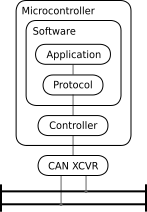
\includegraphics{graphics/canbus_setup}
	\caption{CAN node architecture}
	\label{fig:canbus_setup}
\end{figure}

Starting from the bottom: The CAN bus itself.is a differential signal bus, meaning that the absolute value of each wire in the bus doesn't matter, but the difference between them matters. 
The bus has to be made of twisted pair wires with a characteristic impedance of $\si{120 \ohm}$, and terminated at each end with a $\si{120 \ohm}$ resistor.
That means, that if the bus is broken at any point, no communication will work, even if two nodes are still connected.
Alternately, it is possible to terminate each node, but this greatly reduces transmission speed.\\

The transceivers translate a Tx voltage signal to the differential CAN signal, and simultaneously translates the bus signal to Rx voltage signal. 
For this reason, it is not possible to implement this in most if not all microprocessors.
Because the CAN bus is differential, a transceiver would be able to read the signal it's putting out itself, but they do not transmit these to the Rx pin of the controller.
Other than this blocking of its own signal, it will translate whatever the controller puts out with.
The can transceivers CAN be bought online, but due to the simplicity of this circuitry, the group has designed and manufactured their own.\\

The CAN controller can be standalone hardware, or in many cases be built into the microprocessor.
The major advantage with having the controller built into the microprocessor is, that it would not otherwise require another protocol to communicate between the microprocessor and controller. 
The controller has an input and output FIFO, meaning that the CAN bus communication is asynchronous. 
This is necessary as there is only one bus, and it is likely that there will be a queue of nodes trying to write to the bus.

The protocol in this case refers to a protocol running on top of CAN.
One clear option is the CANopen, which will also be discussed later because it is needed to communicate with the Sevcon. 
Another option is to create our own protocol. 
Because of the specifications for this project, it would be more suitalbe to create our own protocol.
The CANopen encompasses a lot of data registers and addresses, that can be written to and read from, and it definitely lives up to the requirements.
But it is possible to design a high level protocol, that is easy to learn, and has less overhead than CANopen.
This protocol will be described in section~\ref{sub:CAN_protocol}.\\

\subsection{Wireless transmission}
The wireless transmission between the go-kart computer and the stationary computer could be a number of different technologies.
This section seeks to find an appropriate one.

\subsubsection{Range}
The range of the transmission is determined by the length of the test track. 
Normally the SDU kart is tested on parking lots with a maximum lenght of 50m and width of 20m.
There are almost no obstacles for the transmission on such a parking lot. 
This test track sets a minimum requirement that the wireless setup should be able to transmit data at 55m with no obstacles.
\\
At some point it would be interesting to test the go-kart on a real go-kart track. 
The nearest go-kart track is \textit{Odense gokart Hal}, which is also thought to be an average indoor go-kart track.
The track is about 70m long and 40m in width with no obstacles other than the barriers. 
If the wireless transmitter and receiver are placed above the barrier then they will not an obstruction on the transmission. 
This track sets a minimum requirement of 80m transmission. 

\subsubsection{Speed}
The transferred data is from xx sensors producing a maximum of yy bites per sample. 
Data is only used for human inspection and therefore a sample frequency of 100Hz would be sufficient.
This gives a minimum requirement for the speed of the transmission to be ZZ Mbit/s. 

\subsubsection{Compatibility}
It should be possibly to change the stationary computer and therefore the chosen wireless transmission technology should be compatible with standard computers running linux.
The chosen hardware should be compatible with standard linux computers and the Zybo board. 
Both have USB ports and Ethernet ports as a standard, therefore the chosen hardware should one of those.
\todo[inline]{Mikkel: Remove about Zybo}

\subsubsection{Technologies}
Bluetooth is a technology that is compatible with standard computers running linux. 
Bluetooth 5.0 has a maximum speed of 50Mbit/s, which is sufficient.
The range of typical class 2 Bluetooth device is 10m \footnote{https://en.wikipedia.org/wiki/Bluetooth}.
This range is definitely not enough for this application.
\\
\\  
WiFi is also compatible with standard computers running linux and typical WiFi units has speeds that is a lot higher than the required. 
WiFi can be operating in the 2.4GHz band and in the 5GHz band. 
2.4GHz units has the highest range. 
The 802.11n protocol generally has the best range compared to the other 802.11 protocols \footnote{https://en.wikipedia.org/wiki/IEEE\_802.11\#802.11n}.
\\
A local network between computers without connection to existing networks such as the internet is referred to as an ad-hoc network. 
It is a required that the found hardware is capable of doing an ad-hoc network.

\subsubsection{Conclusion} 

\begin{table}[]
\centering
\caption{Minimum requirements for wireless transmission.}
\label{tab:req_wifi}
\begin{tabular}{|l|}
\hline
80m transmission range       \\ \hline
ZZ Mbit/s                    \\ \hline
802.11n protocol             \\ \hline
USB or Ethernet              \\ \hline
ad-hoc network compatability \\ \hline
\end{tabular}
\end{table}
Based on the requirements in table \ref{tab:req_wifi} it was chosen to us the TP-LINK TL-WN722N, as it uses the 2.4GHz band, the 802.11n protocol, is compatible with linux, has an external antenna and uses USB. 






















\subsection{UI}
Somewhere this should be answered!












\subsection{Local Storage}
Somewhere this should be answered!

How should local data storage be realised?

	


% section system_analysis (end)